\documentclass[serif,9pt]{beamer}
\usepackage{color,listings}
\usepackage{ragged2e}
\usepackage[spanish]{babel}
\usepackage[utf8]{inputenc}
\usepackage{graphicx}

\definecolor{dkgreen}{rgb}{0,0.6,0}
\definecolor{gray}{rgb}{0.5,0.5,0.5}
\definecolor{mauve}{rgb}{0.58,0,0.82}
\definecolor{lgray}{rgb}{0.99,0.97,0.95}
\newcommand{\X}{\textbf{X}}
\newcommand{\Y}{\textbf{Y}}
\newcommand{\Z}{\textbf{Z}}
\newcommand{\G}{\textbf{G}}
\newcommand{\R}{\textbf{R}}
\newcommand{\V}{\textbf{V}}
\newcommand{\Q}{\textbf{Q}}
\newcommand{\h}{\textbf{H}}
\newcommand{\T}{\textbf{T}}

\def\E{\mathbb{E}}
\def\C{\mathbb{C}}
\def\N{\mathbb{N}}

\setbeamercovered{transparent}


\usetheme{Frankfurt}
%\usecolortheme{rose}
%\usecolortheme{lily}
\usepackage{amsmath, multirow}
%\usepackage{color, amsmath, wrapfig, anysize, graphicx, hyperref, amsthm, fancyhdr, amssymb,geometry,amsfonts,float}

\newcommand{\ds}{\displaystyle}


\titlegraphic{
\includegraphics[width=4cm]{utfsm.eps}}%
   %\includegraphics[width=4cm]{fig/inria.eps}}

\begin{document}
\title{Presentación de Seminario de Tesis I\\ Hacia una Arquitectura de Referencia de Seguridad del Web Browser} 
\author[Paulina Silva Ghio]{\textsc{Paulina Silva Ghio} \\ \medskip
\small{}
\medskip
\url{pasilva@alumnos.inf.utfsm.cl}}
\institute[]{}
\date{15-01-2016.}

\begin{frame}[plain]
\titlepage
\end{frame}


\begin{frame}
\frametitle{Indice}
\tableofcontents
\end{frame} 


\section{Introducci\'on}
\subsection{Contexto}
\begin{frame}
	\frametitle{Contexto}

	\begin{itemize}
		\item La guerra de los Navegadores: construir y parchar.
		\item El navegador web: herramienta de uso cotidiano.
		\item El usuario com\'un utiliza servicios.
		\item Distintos tipos, distintas implementaciones.
		\item Web 2.0 y 3.0: AJAX (Asynchronous Javascript and XML).
	\end{itemize}
	\begin{figure}[h]
	    \centering
	    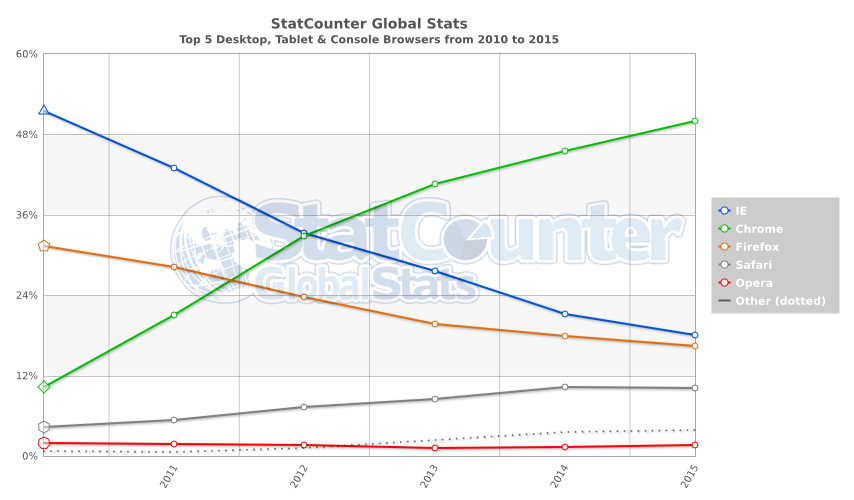
\includegraphics[scale=0.3]{figures/StatCounter-browser-ww-yearly-2010-2015.png}
	    \caption{Porcentaje de uso de Navegadores. Fuente: \cite{statBrow}}
	    \label{fig:UsageShare}
	\end{figure}
\end{frame}

% \subsection{Actualidad}
% \begin{frame}
% 	\frametitle{Actualidad}
% 	\begin{itemize}
% 		\item Sistemas actuales son muy complejos.
% 		\item Es necesario utilizar metodologías que aseguren: Requerimientos Funcionales y No-Funcionales.
% 		\item Defectos y errores en el Software generan vulnerabilidades.
% 		\item La Seguridad es un costo ``extra", a veces no considerado.
% 	\end{itemize}
% 	\begin{block}{Las vulnerabilidades...}
% 		Ocurren por que no se ha tomado en cuenta la seguridad en el desarrollo.
% 	\end{block}
% \end{frame}

\subsection{Motivaci\'on para estudiar el Browser}
\begin{frame}
	\frametitle{Motivaci\'on para estudiar el Browser}
	\onslide{El browser es una herramienta indispensable, \'este permite:}
	\begin{itemize}
		\item Nuevas formas de interactuar.
		\item Disminuir los costos de construir un programa Cliente (desde cero) para
el usuario del sistema.
		\item Seguridad, la que est\'a implementada en los Web Browser es bastante buena.
		\item Es una herramienta indispensable, por lo tanto el reuso es lógico.
	\end{itemize}
	
	\begin{block}<2->{Las preocupaciones principales}
	\begin{itemize}
		\item Los sistemas a los que un usuario hace referencia, y son llamados desde un Web Browser.
		\item Los stakeholders afectados: el usuario del Browser, el Host del usuario y hasta el Servicio externo usado.
	\end{itemize}
	\end{block}
\end{frame}

\section{El Problema}
\subsection{Amenazas y Vulnerabilidades}
\begin{frame}
	\frametitle{Amenazas y Vulnerabilidades}
	\begin{columns}
	\column{0.5\textwidth}
	\begin{minipage}[c][0.4\textheight][c]{\linewidth}
	  \centering
	  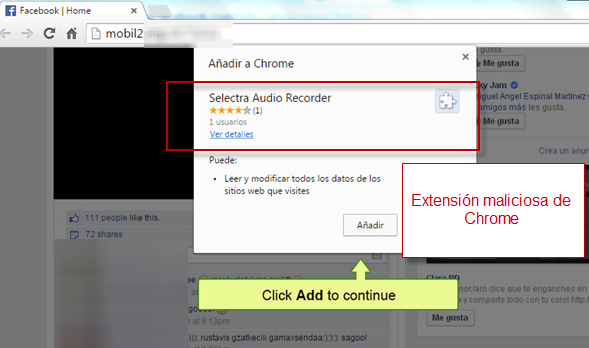
\includegraphics[scale=0.3]{figures/fbporn3.png}
	  \label{fig:Malware}
	\end{minipage}
	\begin{minipage}[c][0.4\textheight][c]{\linewidth}
	  \centering
	  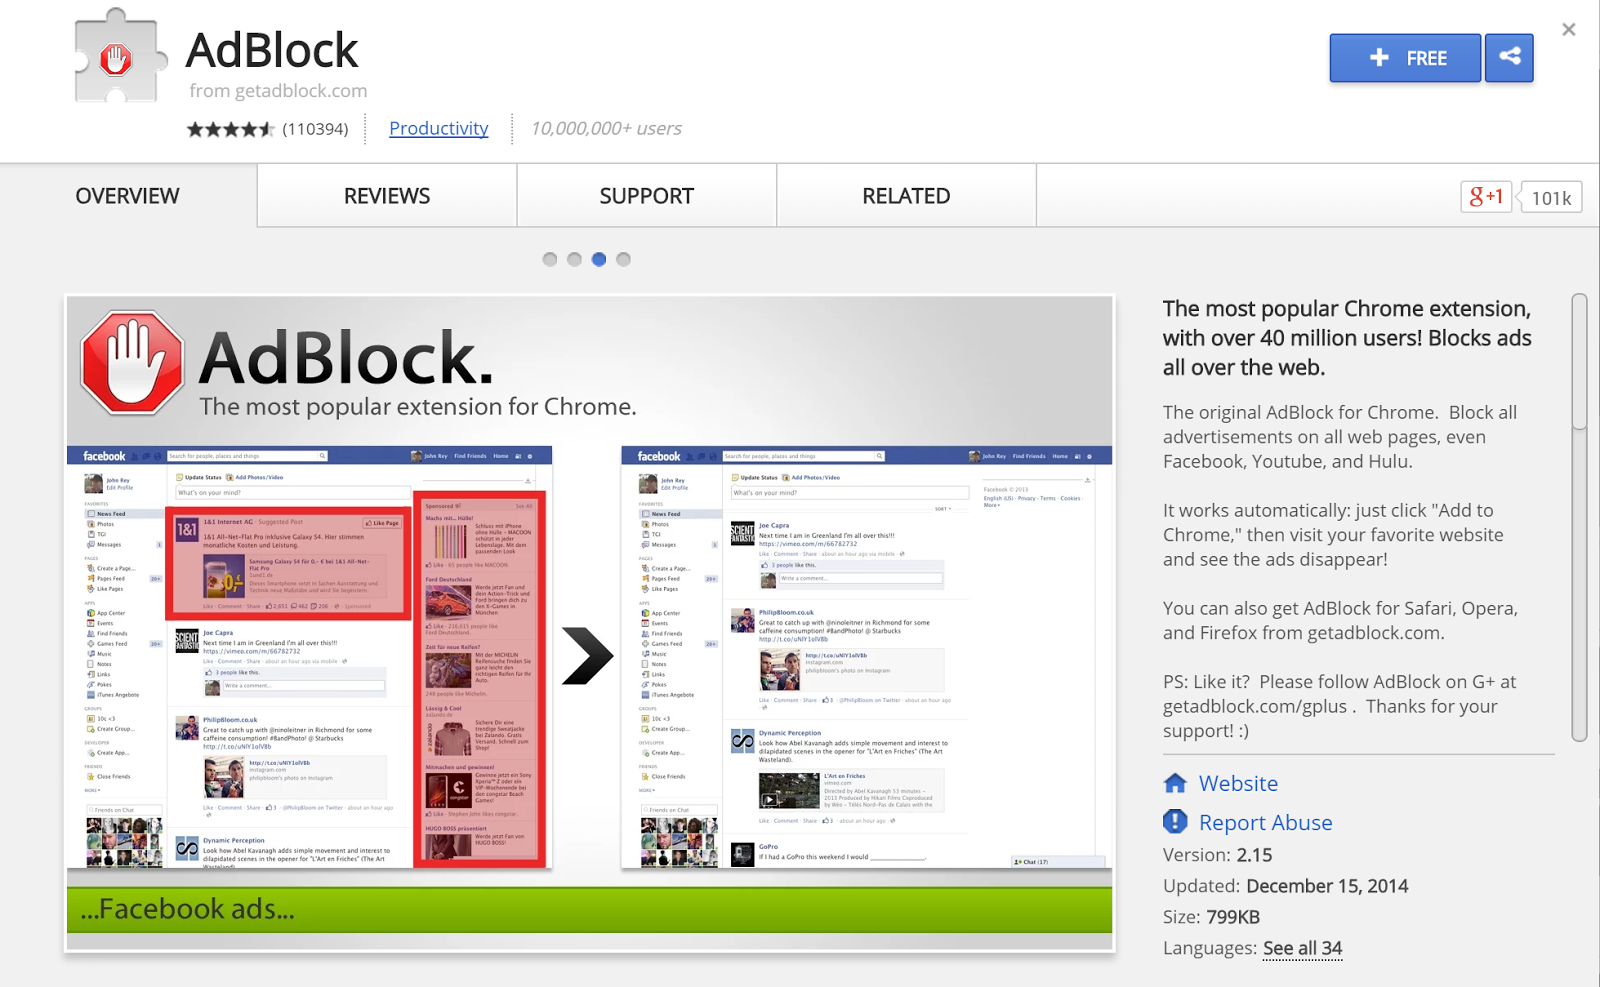
\includegraphics[scale=0.10]{figures/Adblock.png}
	  \label{fig:vulnExt}
	\end{minipage}
	\column{0.5\textwidth}
	\begin{minipage}[c][0.4\textheight][c]{\linewidth}
	  \begin{enumerate}
	  \item Instalaci\'on de Malware o extensiones maliciosas.
	  \item Extensiones Vulnerables.
	  \item Man in the Browser.
	  \item Inyección de código.
	  \end{enumerate}
	\end{minipage}
	\begin{minipage}[c][0.4\textheight][c]{\linewidth}
	  \centering
	  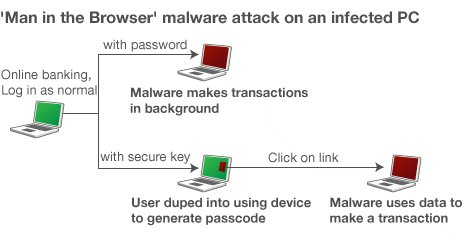
\includegraphics[scale=0.45]{figures/_58291188_malware_464v2.jpg}
	\end{minipage}
	\end{columns}
\end{frame}

\subsection{Problemas}
\begin{frame}
	\frametitle{Problemas}
	\begin{itemize}
		\item<1-> Falta de conocimientos de seguridad con respecto al Browser, podr\'ia afectar de forma directa el desarrollo de aplicaciones que lo utilizan y Stakeholders. 
		\item<2-> Poca documentaci\'on y no hay conceptos unificados. No se ve que existan descripciones formales para los conceptos relacionados al browser.
	\end{itemize}
\end{frame}

\section{Marco Teórico}
\subsection{Arquitectura de Referencia (AR)}
\begin{frame}
	\frametitle{Arquitectura de Referencia (AR) para el browser}
		\begin{itemize}
			\item<1> Especifica la decomposici\'on del sistema en subsistemas, las interacciones entre estas partes y la distribuci\'on de funcionalidad entre ellas. 
			\item<1> Captura la esencia de la arquitectura a trav\'es de una colecci\'on de sistemas similares, por medio del reuso arquitect\'onico.
			\item<1> Actualmente no hay un consenso de cómo definir una AR, lo que debería contener y cómo debería de construirse. En este trabajo usaremos patrones arquitecturales para su construcción.
			\item<2> Describe los Stakeholders que interactuan con el sistema y que poseen preocupaciones/concerns de \'este, así como los atributos de calidad deseables que el sistema debe garantizar.
			\item<2> Ayuda: 1) a los implementores o desarrolladores del software, a entender los trade-off cuando se diseñan nuevos sistemas, 2) a los mantenedores de estos sistemas a entender el c\'odigo legacy usado.
			\item<2> Comparar las diferencias en decisiones de diseño y poder entender los cambios realizados a lo largo del Desarrollo de un sistema.
			\item<3> Mirada hol\'istica del Sistema.
		\end{itemize}
	\begin{block}<4>{Desventajas}
		Incluso realizar los casos de uso más importantes del sistema toma tiempo.
	\end{block}
\end{frame}

\subsection{Arquitectura de Referencia de Seguridad (ARS)}
\begin{frame}
	\frametitle{Arquitectura de Referencia de Seguridad (ARS) para el browser}
	\begin{itemize}
		\item<1> Abtracción de los mecanismos de defensa en forma de patrones de seguridad
		\item<1> Se enseña en que lugares de la Arquitectura de Referencia son necesitados.
		\item<1> Una forma de entender y descomponener un sistema complejo con mecanismos de defensa que aumentan esa complejidad.
		\item<2> Una vista holística de la seguridad, teniendo en cuenta las interacciones con otros sistemas que pueden generar vulnerabilidades.
		\item<2> Unifica la terminología. Esto permite comparar diferentes implementaciones bajo las mismas definiciones de conceptos.
		\item<2> Evaluación de la seguridad del browser
		\item<3> Selección de un browser basado en los requerimientos de seguridad.
		\item<3> Referencia para funciones de monitoreo y forense.
	\end{itemize}
	\begin{block}<4>{Desventajas}
		\begin{itemize}
			\item Se necesita invertir mucho tiempo en la construcción, al menos de los componenentes más importantes.
		\end{itemize}
	\end{block}
\end{frame}

\subsection{Patrones del Mal Uso}
\begin{frame}
	\frametitle{Patrones del Mal Uso}
	\begin{itemize}
		\item Describen desde el punto de vista del atacante, como un tipo de ataque es realizado (que unidades usa y cómo), analiza las formas de detener el ataque enumerando los posibles patrones de seguridad qu pueden ser utilizados, y describe como rastrear el ataque una vez ocurrido con la recolección y observación de datos forenses.
		\item Permitir\'an enseñar y comunicar las posibles formas en que tal sistema puede ser usado inapropiadamente.
		\item Normalmente explicado a traves de un diagrama de secuencia o colaboración: es posible relacionar los mensajes con los componentes que los reciben.
	\end{itemize}
\end{frame}


\subsection{Estado del Arte}
\begin{frame}
	\frametitle{Estado del Arte}
	\begin{itemize}
		\item No se encontr\'o informaci\'on actualizada sobre una Arquitectura de Referencia del Browser. Hay una \cite{preprint-grosskurth-browser-archevol}, pero es muy antigua.
		\item Trabajos encontrados: 
		\begin{itemize}
			\item<1-> Larrondo et al. \cite{535061}: análisis del web browser, con el fin de obtener un Modelo de Dominio, un Modelo de Objetos y un Feature Tree que describiera la estructura y funcionalidad entregada comúnmente por los Web Browser.
			\item<2-> Grosskurth et al. \cite{2005-grosskurth-browser-refarch,preprint-grosskurth-browser-archevol}: utiliza una herramienta de ingeniería inversa, para obtener una arquitectura de referencia de muy alto nivel en base a dos navegadores open-source: Mozilla y Konqueror.
			\item<3-> Godfrey et al. \cite{Godfrey2000}: se extrajo la arquitectura de software del Navegador Mozilla, con el objetivo de entender la estructuración de sus componentes; además de crear vistas arquitecturales de alto nivel del sistema.
			\item<4-> Lwin \cite{Lwin2009}]: propone un Browser llamado Anfel SOFT, donde gracias al uso de Inteligencia Artificial, crea agentes que permiten mejorar la experiencia del usuario.
		\end{itemize}
		\item Poca documentaci\'on y no hay conceptos unificados.
		\item Queda por buscar si existe algo parecido a una Arquitectura de Referencia de Seguridad del Browser.
	\end{itemize}
\end{frame}


\section{Propuesta}
\subsection{Objetivo General y Específicos}
\begin{frame}
	\frametitle{Objetivo General y Específicos}
	\begin{block}{Objetivo General}
		\begin{small}
		\begin{itemize}
			\item Generar un cuerpo organizado de informaci\'on sobre el Web Browser y su seguridad.
			\item Sistematizar, organizar y clasificar el conocimiento adquirido en un documento, con formato semi-formal. 
			\item Lograr una mejor comprensión sobre la seguridad en el web browser.
		\end{itemize}
		\end{small}
	\end{block}
	\begin{block}<2->{Objetivos Espec\'ificos}
		\begin{small}
			\begin{itemize}
				\item Una gu\'ia para comunicar los conceptos relevantes que pudieran afectar la relaci\'on existente entre un desarrollo de software y el navegador. 
				\item Mejorar la Arquitectura de Referencia (AR) obtenida en la memoria de Pregrado para agregar más patrones a ésta y continuar el cat\'alogo de Patrones de Mal Uso. 
				\item Construir un modelo conceptual de la seguridad del web browser a través de una Arquitectura de Referencia de Seguridad, identificando patrones de seguridad en el navegador.
				\item Profundizar el conocimiento en ataques relacionados con m\'etodos de Ingenier\'ia Social.
				\item Utilizar técnicas de Ingeniería de Software Experimental.
			\end{itemize}
		\end{small}
	\end{block}
\end{frame}


\subsection{Hipótesis}
\begin{frame}
	\frametitle{Hipótesis}	
	\begin{block}{Hipótesis Principal}
			H1: La definición de una Arquitectura de Referencia de Seguridad para web browsers permite abstraer y capturar los principales aspectos estructurales y de comportamiento de éstos, facilitando la expresión de los patrones más conocidos de mal uso y seguridad relacionados con los navegadores.
	\end{block}
	% \begin{block}{Otra posible hipótesis}
	% 	%\begin{itemize}
	% 	H2: El uso de una Arquitectura de Referencia de Seguridad permite añadir seguridad al desarrollo de aplicaciones web.
	% 		%\item H3: El uso de una Arquitectura de Referencia de Seguridad permite la construcción de Browser Seguros.
	% 	%\end{itemize}
	% \end{block}
\end{frame}

\subsection{Formas de Validación}
\begin{frame}
	\frametitle{Formas de Validación}	
	\begin{itemize}
	\item<1-> Las Arquitecturas de Referencias (AR/RA) y Arquitecturas de Referencias de Seguridad (ARS/SRA) no son implementables. Éstos son modelos abstractos y no pueden ser evaluados con respecto a la seguridad o desempeño por medio de testing o experimentación.
	\item<1-> La validación de los artefactos generados en este trabajo será a través de la revisión realizada por expertos en el área de computer science y patrones, por medio de la asistencia de conferencias. 
	\item<2-> Al ser aceptados, presentados, mejorados y publicados en conferencias *PLoP, tendremos un respaldo de la utilidad de estos patrones. Los patrones antes de ser publicados, son refinados a través del proceso llamado ``Shepherding". Para esta tesis se espera ir a las conferencias: AsianPLoP y EuroPLoP.
	\item<2-> Se utilizarán conocimientos en ingeniería de software experimental para probar nuestra hipótesis. 
	\end{itemize}
\end{frame}

\subsection{Trabajo Adelantado}
\begin{frame}
	\frametitle{Trabajo Adelantado}
	\begin{itemize}
		\item En la memoria de Pregrado se obtuvo un Estado del Arte sobre el Browser y documentación sobre Arquitecturas de Referencias existntes. Falta averiguar sobre Arquitecturas de Referencia de Seguridad.
		\item Se han enviado 2 papers a la conferencia AsianPLoP con lo obtenido en la memoria de pregrado. El proceso llamado ``shepherding" permite evaluar el paper enviado, al mismo tiempo que provee al autor la mejora del trabajo a través del intercambio continuo de sugerencias entre el autor/autores con el ``shepherd".
	\end{itemize}
\end{frame}

\section{Metodología y Plan de Trabajo}
\begin{frame}
	\frametitle{Metodología y Plan de Trabajo}
	\begin{itemize}
		\item Marco teórico y Estado del Arte: Revisión de conceptos relevantes del navegador, seguridad y Arquitecturas de Referencias existentes.
		\item Evaluación de Resultados Intermedios: a) Envío de papers a Asian PLoP, b) Depurar el modelo obtenido en la memoria de pregrado.
		\item Agregar nuevos patrones y adecuar modelo para especificar semi-formalmente estos patrones. Creación de la Arquitectura de Referencia de Seguridad.
		\item Producir segunda versión de publicaciones: Se enviarán más trabajos a conferencias de tipo PLoP (Pattern Languages of Programs), la siguiente más próxima es el EuroPLoP.
		\item Documentar la tesis a partir de la compilación de papers obtenidos y el trabajo adelantado.
	\end{itemize}

	\begin{table}
        \begin{tabular}{|c|c|} 
        \hline        
        \textbf{Actividad} & \textbf{Fecha}\\
        \hline
        Marco teórico y Estado del Arte & Noviembre 2015 - Enero 2016\\
        \hline
        Evaluación de Resultados Intermedios & Noviembre 2015  - Febrero 2016\\
        \hline
        Agregar nuevos patrones y adecuar modelo & Enero - Abril 2016\\
        \hline
        Producir segunda versión de publicaciones & Enero - Junio 2016\\
        \hline
        Documentar la tesis & Enero - Junio 2016\\        
        \hline
        \end{tabular}
        \caption{Plan de Trabajo}
        \label{tab:trabajo}
    \end{table}
\end{frame}

\section{Aportes y Resultados Esperados}
\begin{frame}
	\frametitle{Aportes y Resultados Esperados}
	\begin{itemize}
		\item Se espera poder obtener una documentación semi-formal que permita comprender mejor la seguridad y estructura del browser. Para así entender que éste tiene una superficie de ataque muy usada por los atacantes de los sistemas con los que se conecta el usuario, utilizando frecuentemente ataques de ingeniería social.
		\item Crear un catálogo de patrones de mal uso que permitan instruir a personas en el área de IT pero carecen de conocimientos de seguridad, sobre los tipos de ataques existentes.
		\item Arquitecturas de Referencia (AR) de su infraestructura como de los mecanismos de defensa existentes (ARS). Incluyendo 2 nuevos patrones arquitecturales: el Browser Kernel y el Web Content Renderer. Patrones de Seguridad existentes o nuevos y aún no documentados.
		\item Experimentación del modelo utilizando técnicas de ingeniería de software experimental.
	\end{itemize}
\end{frame}


\begin{frame}
	\frametitle{¿Preguntas?}
	¡Muchas Gracias!	
\end{frame}

\bibliography{refTodas}
\bibliographystyle{IEEEtran}

\end{document}

